\documentclass[journal,12pt,twocolumn]{IEEEtran}
\usepackage{setspace}
\usepackage{gensymb}
\singlespacing
\usepackage[cmex10]{amsmath}
\usepackage{amsthm}
\usepackage{mathrsfs}
\usepackage{txfonts}
\usepackage{stfloats}
\usepackage{bm}
\usepackage{cite}
\usepackage{cases}
\usepackage{subfig}
\usepackage{longtable}
\usepackage{multirow}
\usepackage{enumitem}
\usepackage{mathtools}
\usepackage{steinmetz}
\usepackage{tikz}
\usepackage{circuitikz}
\usepackage{verbatim}
\usepackage{tfrupee}
\usepackage[breaklinks=true]{hyperref}
\usepackage{graphicx}
\usepackage{tkz-euclide}
\usetikzlibrary{calc,math}
\usepackage{listings}
    \usepackage{color}                                            %%
    \usepackage{array}                                            %%
    \usepackage{longtable}                                        %%
    \usepackage{calc}                                             %%
    \usepackage{multirow}                                         %%
    \usepackage{hhline}                                           %%
    \usepackage{ifthen}                                           %%
    \usepackage{lscape}     
\usepackage{multicol}
\usepackage{chngcntr}
\DeclareMathOperator*{\Res}{Res}
\newcommand{\myvec}[1]{\ensuremath{\begin{pmatrix}#1\end{pmatrix}}}
\renewcommand\thesection{\arabic{section}}
\renewcommand\thesubsection{\thesection.\arabic{subsection}}
\renewcommand\thesubsubsection{\thesubsection.\arabic{subsubsection}}
\renewcommand\thesectiondis{\arabic{section}}
\renewcommand\thesubsectiondis{\thesectiondis.\arabic{subsection}}
\renewcommand\thesubsubsectiondis{\thesubsectiondis.\arabic{subsubsection}}
\hyphenation{op-tical net-works semi-conduc-tor}
\def\inputGnumericTable{}                                 %%
\lstset{
%language=C,
frame=single, 
breaklines=true,
columns=fullflexible
}
\begin{document}
\newtheorem{theorem}{Theorem}[section]
\newtheorem{problem}{Problem}
\newtheorem{proposition}{Proposition}[section]
\newtheorem{lemma}{Lemma}[section]
\newtheorem{corollary}[theorem]{Corollary}
\newtheorem{example}{Example}[section]
\newtheorem{definition}[problem]{Definition}
\newcommand{\BEQA}{\begin{eqnarray}}
\newcommand{\EEQA}{\end{eqnarray}}
\newcommand{\define}{\stackrel{\triangle}{=}}
\bibliographystyle{IEEEtran}
\providecommand{\mbf}{\mathbf}
\providecommand{\pr}[1]{\ensuremath{\Pr\left(#1\right)}}
\providecommand{\qfunc}[1]{\ensuremath{Q\left(#1\right)}}
\providecommand{\sbrak}[1]{\ensuremath{{}\left[#1\right]}}
\providecommand{\lsbrak}[1]{\ensuremath{{}\left[#1\right.}}
\providecommand{\rsbrak}[1]{\ensuremath{{}\left.#1\right]}}
\providecommand{\brak}[1]{\ensuremath{\left(#1\right)}}
\providecommand{\lbrak}[1]{\ensuremath{\left(#1\right.}}
\providecommand{\rbrak}[1]{\ensuremath{\left.#1\right)}}
\providecommand{\cbrak}[1]{\ensuremath{\left\{#1\right\}}}
\providecommand{\lcbrak}[1]{\ensuremath{\left\{#1\right.}}
\providecommand{\rcbrak}[1]{\ensuremath{\left.#1\right\}}}
\theoremstyle{remark}
\newtheorem{rem}{Remark}
\newcommand{\sgn}{\mathop{\mathrm{sgn}}}
\providecommand{\abs}[1]{\vert#1\vert}
\providecommand{\res}[1]{\Res\displaylimits_{#1}} 
\providecommand{\norm}[1]{\Vert#1\rVert}
%\providecommand{\norm}[1]{\lVert#1\rVert}
\providecommand{\mtx}[1]{\mathbf{#1}}
\providecommand{\mean}[1]{E[ #1 ]}
\providecommand{\fourier}{\overset{\mathcal{F}}{ \rightleftharpoons}}
%\providecommand{\hilbert}{\overset{\mathcal{H}}{ \rightleftharpoons}}
\providecommand{\system}{\overset{\mathcal{H}}{ \longleftrightarrow}}
	%\newcommand{\solution}[2]{\textbf{Solution:}{#1}}
\newcommand{\solution}{\noindent \textbf{Solution: }}
\newcommand{\cosec}{\,\text{cosec}\,}
\providecommand{\dec}[2]{\ensuremath{\overset{#1}{\underset{#2}{\gtrless}}}}
\newcommand{\myvec}[1]{\ensuremath{\begin{pmatrix}#1\end{pmatrix}}}
\newcommand{\mydet}[1]{\ensuremath{\begin{vmatrix}#1\end{vmatrix}}}
\numberwithin{equation}{subsection}
\makeatletter
\@addtoreset{figure}{problem}
\makeatother
\let\StandardTheFigure\thefigure
\let\vec\mathbf
\renewcommand{\thefigure}{\theproblem}
\def\putbox#1#2#3{\makebox[0in][l]{\makebox[#1][l]{}\raisebox{\baselineskip}[0in][0in]{\raisebox{#2}[0in][0in]{#3}}}}
     \def\rightbox#1{\makebox[0in][r]{#1}}
     \def\centbox#1{\makebox[0in]{#1}}
     \def\topbox#1{\raisebox{-\baselineskip}[0in][0in]{#1}}
     \def\midbox#1{\raisebox{-0.5\baselineskip}[0in][0in]{#1}}
\vspace{3cm}
\title{ASSIGNMENT-2}
\author{Ojaswa Pandey}
\maketitle
\newpage
\bigskip
\renewcommand{\thefigure}{\theenumi}
\renewcommand{\thetable}{\theenumi}
Download all python codes from 
\begin{lstlisting}
https://github.com/behappy0604/Summer-Internship-IITH/tree/main/Assignment-3
\end{lstlisting}
%
and latex-tikz codes from 
%
\begin{lstlisting}
https://github.com/behappy0604/Summer-Internship-IITH/tree/main/Assignment-3
\end{lstlisting}
%
\section{Question No. 2.60}   
Let ABC be a right triangle in which $a = 8, c = 6$ and $\angle B = 90^{\degree}$.  $BD$ is the 
perpendicular from $\vec{B}$ on $AC$ (altitude). The circle through $\vec{B}, \vec{C}, \vec{D}$ (circumcircle of $\triangle BCD$) is drawn.  Construct the 
tangents from $\vec{A}$ to this circle.
\section{Solution}
Data from the given question 
\numberwithin{table}{section}
\begin{table}[!ht]
\begin{center}
\begin{tabular}{ | m{2cm} | m{1.5cm}| m{2cm} | m{1.5cm} |} 
\hline
& Symbols & Circle \\
\hline
Centre & $\vec{E}$ & \myvec{4\\0}  \\ 
\hline
Radius & $r_$ & 4 \\ 
\hline
\end{tabular}
\end{center}
\end{table}
\begin{enumerate}
    \item  Let us generalise the given data:
\begin{align}
\vec{B}= \myvec{0\\0}, \vec{A}=\myvec{0\\c}, \vec{C}= \myvec{a\\0}
\end{align}
\begin{align}
    \beta= \angle DBC
\end{align}
\begin{align}
    \alpha= \angle PEC
\end{align}
\begin{align}
\vec{AB}=c
\end{align}
\begin{align}
    \vec{BC}=a
\end{align}
\begin{align}
    \vec{AC}=b
\end{align}
\begin{align}
    \vec{BD}=t
\end{align}
\item Let $\vec{E}$ be the the midpoint of $\vec{BC}$, therefore
\begin{align}
    \vec{E}= \frac{\vec{B}+\vec{C}}{2}= \myvec{\frac{a}{2}\\0}
    \end{align}
    \item Now taking $\vec{E}$ as center we will draw a circle of radius 4 which will circumscribe $\triangle BCD$.\\
    
    \item Tangents to this circle from point $\vec{A}$ will be $\vec{AB}$ and $\vec{AP}$ as shown in the figure.\\
    \item Using sine formula we get,
    \begin{align}
    \angle BAE=33.69\degree
    \end{align}
    \begin{align}
        \angle BAC=53.18\degree
    \end{align}
    \begin{align}
       \vec{BD}= 4.8
    \end{align}
      \begin{align}
        \angle DBC=53.13\degree
    \end{align}
  \item   Now, \begin{align}
        \vec{D}= \vec{B}+\myvec{r\cos \beta\\r\sin \beta}
    \end{align}
    \begin{align}
     \vec{D}= \myvec{0\\0}+\myvec{0.60\\0.799}   
    \end{align}
    \begin{align}
        \vec{D}=\myvec{2.88\\3.84}
    \end{align}
\item Here,
\begin{align}
\angle PEC= 2\angle BAE
\end{align}
\begin{align}
    \angle PEC=2\times 33.69\degree
\end{align}
\begin{align}
    \angle PEC= 67.38\degree
\end{align}
\item Now coordinates of $\vec{P}$ from center of circle $\vec{E}$ will be,
\begin{align}
    \vec{P}= \vec{E}+\myvec{r\cos \alpha\\r\sin \alpha}
\end{align}
\begin{align}
    \vec{P}=\myvec{4\\0}+\myvec{1.53\\3.69}
\end{align}
\begin{align}
    \vec{P}=\myvec{5.53\\3.69}
\end{align}
\item Therefore, we have coordinates as,\\
\begin{multiline}
    $\vec{A}$=$\myvec{0\\6} $,$\vec{B} $= $\myvec{0\\0} $,$\vec{C} $= $\myvec{8\\0} $,  $\vec{E} $= $\myvec{4\\0} $,  $\vec{P}=\myvec{5.53\\3.69} $,\\$\vec{D} $= $\myvec{2.88\\3.84} $\\
\end{multiline}
\item On constructing the given figure we get:
\end{enumerate}
\numberwithin{figure}{section}
\begin{figure}[!ht]
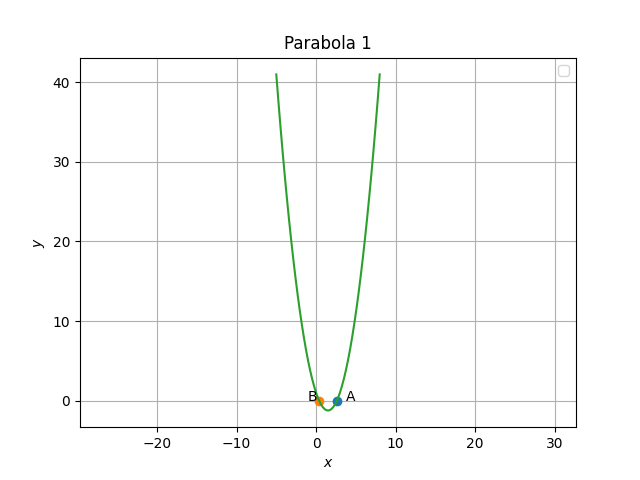
\includegraphics[ width=\columnwidth, height=7 cm]{figure.png}
\caption{Tangents to a Circle}
\label{fig:Circle}	
\end{figure}
\end{document}
